%====================================================================================================
% En-tête
%====================================================================================================
\begin{figure}[H]
    \centering
    \includegraphics[scale=0.65]{assets/figures/Mechanical Design/Système.png}
    \caption{Representation of the Mechanical design}
    \label{fig:Mec_Blobal}
\end{figure}
\newpage
%====================================================================================================
% Preliminary choices and limitations
%====================================================================================================
\section{Preliminary choices and limitations}
\subsection{Objectives}
First, the mechanical system need to be attached to the output of the laboratory telescope. To achieve this, an adaptor piece is
required (\ref{sec:adaptator}). Then, the masks will need to be attached to a support (\ref{sec:mask}). A second support will have
to be made to accommodate the prisms (\ref{sec:prisms}). Finally, the lens must be installed (\ref{sec:lens}) and the camera placed
just behind it (\ref{sec:Camera}). \newline
The system must be compact, adjustable and adaptable if modifications are required at a later date.
\subsection{Limitations}
To make this system a reality, a simple and common fastening system had to be integrated. The most simple system used in optical design 
is the cage system. Two of the world's leading optomechanics manufacturers offer it (Thorlabs and Edmund Optics). The significant difference 
between these 2 manufacturers is the spacing between the steel bars. This difference is shown in the capter \ref{sec:lens}. \newline
To integrate the telescope's occular correctly, the Edmund optics system is required. This is because the distance between the steel bars 
is smaller on the thorlabs system, and the distance between the occular and the bore for the bar would be far too small ($\approx$ 0.05mm).
\bigbreak
The difference between the Thorlabs system and the Edmund Optics system is the centering diameters for the steel bar holes who 
can be seen on the figure \ref{fig:thorlabs_Edmund} ($\emptyset\ 38\ mm$ for Thorlabs (blue) and $\emptyset\ 57\ mm$ for Edmund optics (red))
\begin{figure}[H]
    \centering
    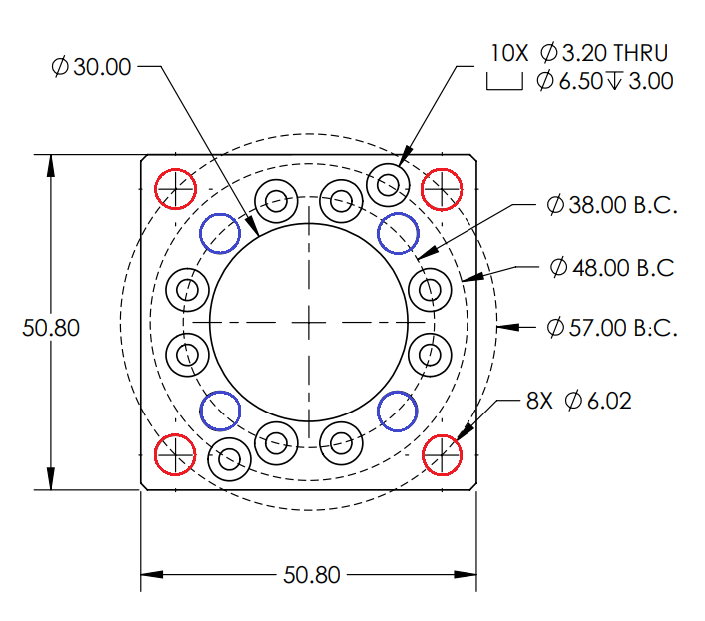
\includegraphics[scale=1]{assets/figures/Mechanical Design/Thorlabs_Edmund.png}
    \caption{Differences between thorlabs and Edmund systems}
    \label{fig:thorlabs_Edmund}
\end{figure}
%====================================================================================================
% Telescope mounting system
%====================================================================================================
\section{Telescope mounting system}\label{sec:adaptator}
The telescope-mounting system, as its name suggests, will be the connecting piece between the telescope output and the DIMM. It will 
also integrate the telescope's occular. The choice of integrating the telescope's ocular with this part was made to improve the system's 
stability and alignment. The system will be screwed onto the telescope, so it won't be held in place by simple screws attached to 
the part. \newline
This part will maintain all the DIMM. So it need to be strong and more massive than the other parts. However, it also needs to be as 
light as possible so as not to weigh too much on the telescope. Material was therefore removed from the middle of the piece to reduce 
its weight.
\bigbreak
Figure \ref{fig:Mec_Adapter1} (Adapter drawing) shows :
\begin{enumerate}
    \item The hole for the ocular ($\emptyset\ 33.55\ mm$) and the thread for its attachment ($MF\ 40\ P=1$). Fixing is simply done 
    with a threaded ring drilled through the center.
    \item The thread for attaching the system to the telescope ($\emptyset\ 50.75\ mm\ TPI\ 24$)
    \item Hole for steel bars and the screws used to secure them ($\emptyset\ 6.02$)
\end{enumerate}
\begin{figure}[H]
    \centering
    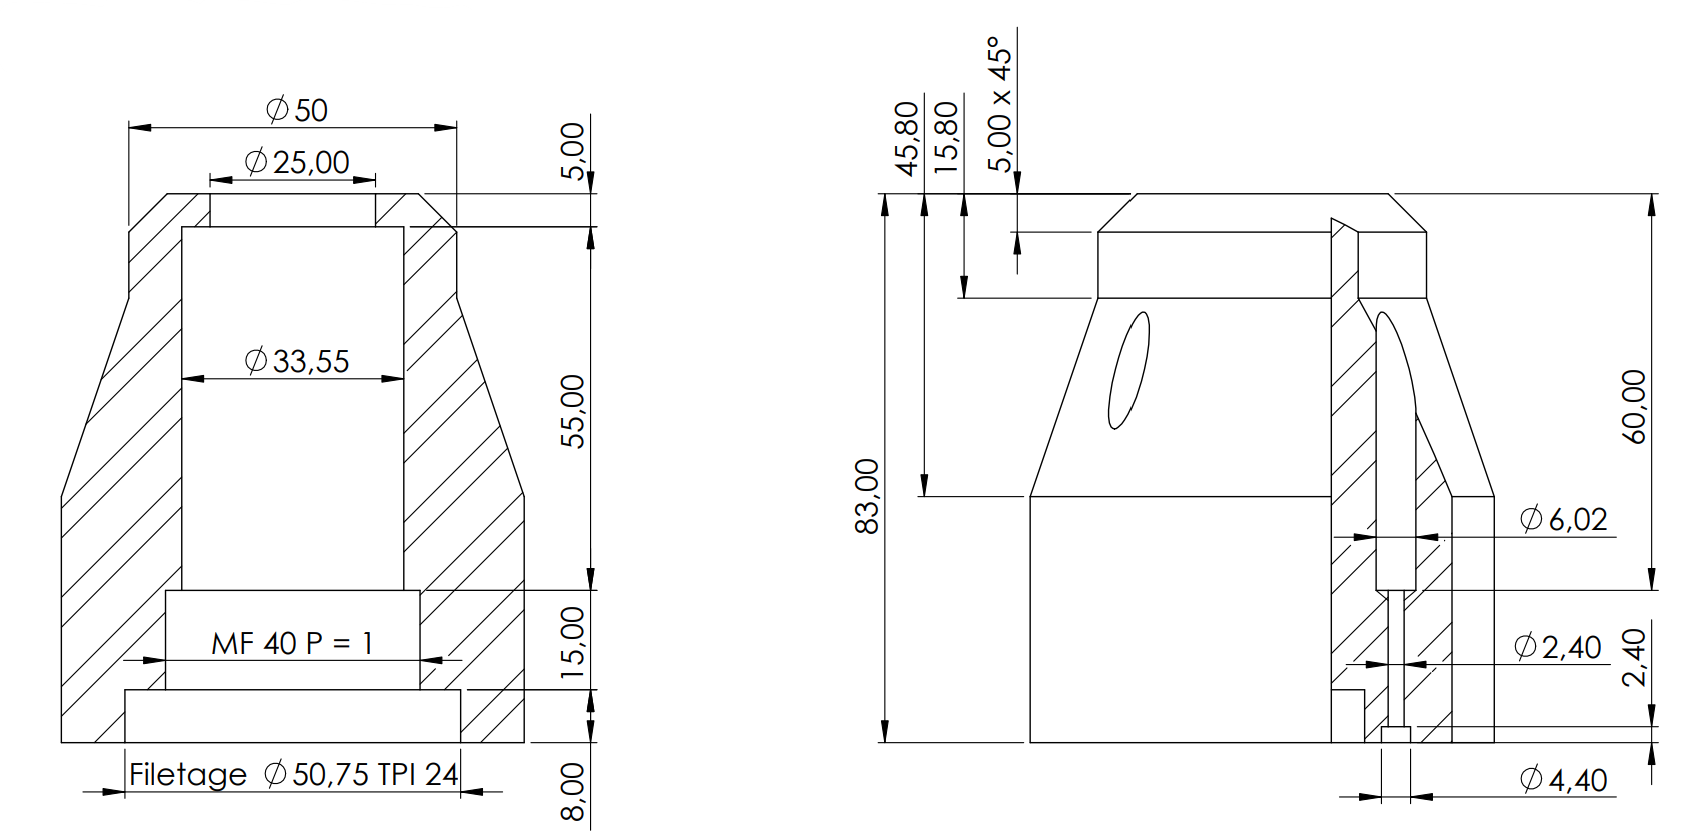
\includegraphics[scale=0.6]{assets/figures/Mechanical Design/Dessin_Part1_adapter.png}
    \caption{Representation of the adaptator : ocular and bar fixation}
    \label{fig:Mec_Adapter1}
\end{figure}
This part will be made of aluminum to reduce its weight. The use of aluminum has no effect on the rigidity of the system. \newline
However, the ocular attachment ring will be made of steel to limit the coefficient of friction when screwing it on 
(screwing an aluminum part with another of this material will have a grip effect between the two parts).
\bigbreak
The complete drawing can be found in the appendix \ref{App:MEP}
\newpage
%====================================================================================================
% Mask mounting
%====================================================================================================
\section{Mask and mounting}\label{sec:mask}
\subsection{Mask}
As explained in section \ref{sec:Opti_Limit}, the mask will have 2 holes 1mm in diameter, with their centers 5mm apart. 
A 0.5mm-thick plate was designed for this purpose. This plate includes the 2 holes and is shaped to fit more easily into its support.
This part is shown in figure \ref{fig:Mec_Mask}
\begin{figure}[H]
    \centering
    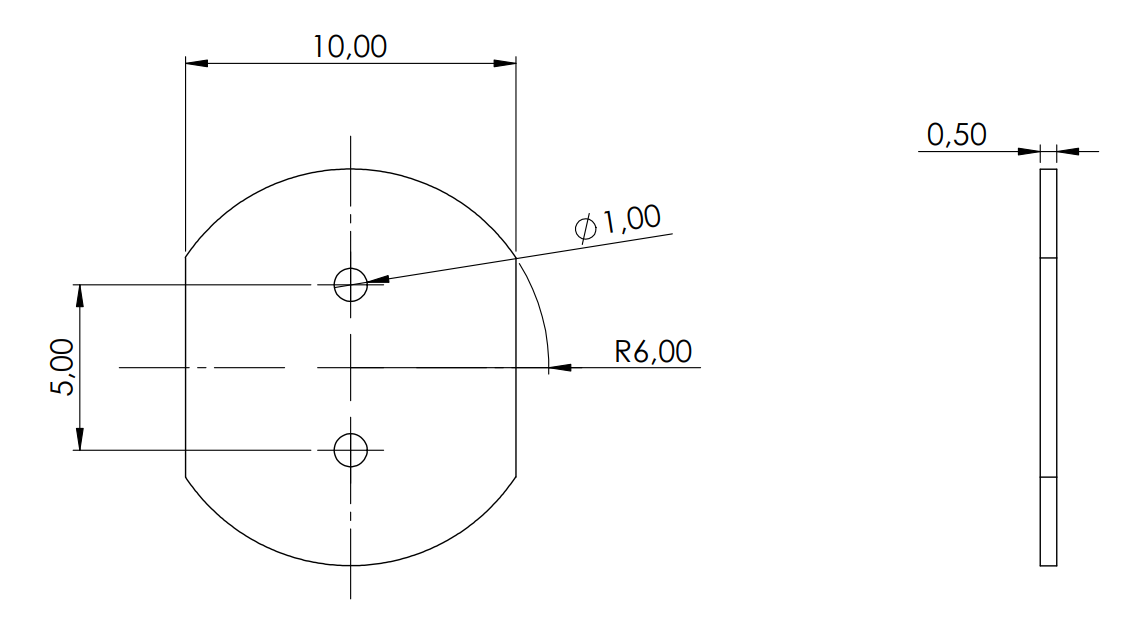
\includegraphics[scale=0.6]{assets/figures/Mechanical Design/Dessin_Mask.png}
    \caption{Drawing of the mask}
    \label{fig:Mec_Mask}
\end{figure}
\subsection{Mounting}
For the support, 2 pieces are required. The first will contain the "rail" where the mask will be inserted (Figure \ref{fig:Mec_Mask_Sup_Rail} left),
 and the other will hold it in place (Figure \ref{fig:Mec_Mask_Sup_Rail} right).
\begin{figure}[H]
    \centering
    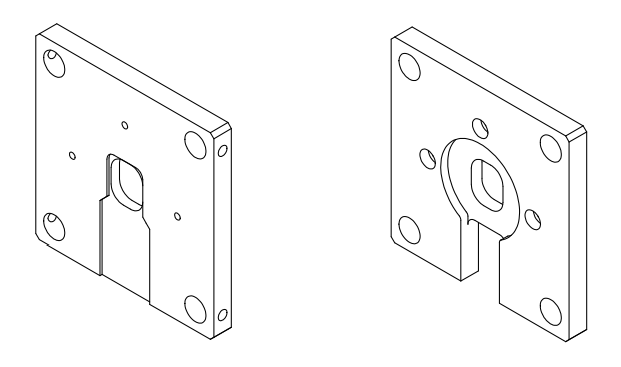
\includegraphics[scale=0.8]{assets/figures/Mechanical Design/Support_masque_rail.png}
    \caption{Drawing of the support ("rail" part)}
    \label{fig:Mec_Mask_Sup_Rail}
\end{figure}
Figure \ref{fig:Mec_Mask_Sup_Rail} (left) shows the mask positioning rail, the tapped holes for attaching the second part and the holes 
for the steel bars. \newline
Figure \ref{fig:Mec_Mask_Sup_Rail} (right) shows the second piece who is designed for easy mask removal. This part also features the opening 
for inserting the mask, as well as the screw holes for securing the two parts together.\bigbreak
This part will be made of aluminum to reduce its weight. The use of aluminum has no effect on the rigidity of the system.
\bigbreak
The complete drawing can be found in the appendix \ref{App:MEP}
%====================================================================================================
% Prisms and mounting
%====================================================================================================
\section{Prisms and mounting}\label{sec:prisms}
\subsection{Prisms}
As explained in section 2, the output beams from the prism must have an angle of incidence of 1°. 
This corresponds to an angle of 1.93° on the prism. \newline
Several requests for bids were made, but none were within the budget allocated under the TB. The aim was to have a square-shaped 
prism (\ref{fig:Prism_square} left) to reduce the size of the system and make it easier to assemble. However, this solution could not be retained and the 
use of circular prisms (\ref{fig:Prism_square} right) was required. This solution greatly reduces the budget, but the part that will hold them will be much more complex.
\begin{figure}[H]
    \centering
    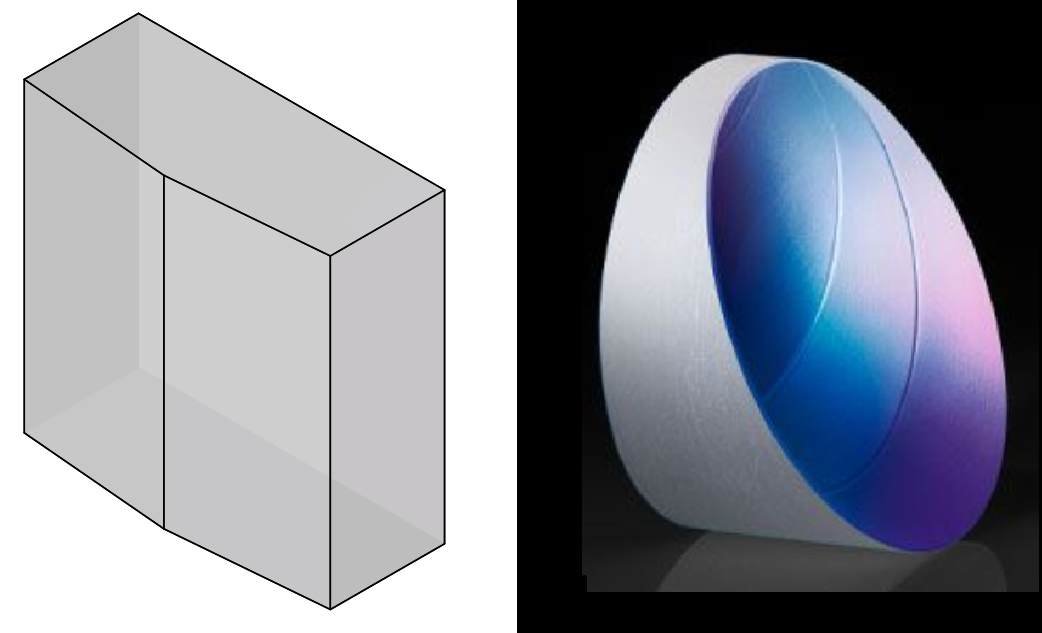
\includegraphics[scale=0.6]{assets/figures/Mechanical Design/prisme_voulu.png}
    \caption{Needed prism / Prism choosed}
    \label{fig:Prism_square}
\end{figure}
\subsection{Mounting}
blablalba
\bigbreak
The complete drawing can be found in the appendix \ref{App:MEP}
%====================================================================================================
% Lens and mounting
%====================================================================================================
\section{Lens and mounting}\label{sec:lens}
\subsection{Lens}
blablablalb
\subsection{Mounting}
test deassdsa adsd asda sd ads a sdasas ads asada ss dd ad s ad aasdasdads 
\bigbreak
The complete drawing can be found in the appendix \ref{App:MEP}
%====================================================================================================
% Camera mounting
%====================================================================================================
\section{Camera mounting}\label{sec:Camera}
blablalbalb
\bigbreak
The complete drawing can be found in the appendix \ref{App:MEP}